%% LLM-Para Paper --- IEEE Access Format
%% Compile: pdflatex -> bibtex -> pdflatex -> pdflatex
%% Template: IEEEtran (double-column, journal)

\documentclass[journal]{IEEEtran}

% ── Packages ──────────────────────────────────────────────────────────────────
\usepackage[T1]{fontenc}
\usepackage[utf8]{inputenc}
\usepackage{amsmath,amssymb,amsfonts}
\usepackage{graphicx}
\usepackage{booktabs}
\usepackage{multirow}
\usepackage{xcolor}
\PassOptionsToPackage{hyphens}{url}
\usepackage{hyperref}
\usepackage{algorithm}
\usepackage{algpseudocode}
\usepackage{subcaption}
\usepackage{siunitx}

\hypersetup{
  colorlinks=true,
  linkcolor=blue,
  citecolor=blue,
  urlcolor=blue
}

% ── Title & Authors ────────────────────────────────────────────────────────────
\title{LLM-Para: A Multi-Metric First-Order Roofline Analysis Framework
       for LLM Inference on Heterogeneous Multi-Tier Memory Architectures}

\author{%
  Lishuo~Deng%
  \thanks{Manuscript received \today.}%
  \thanks{The authors are with [Institution Name], [City, Country].
          E-mail: \texttt{your-email@institution.edu}.}%
  \thanks{Source code and live demo:
          \url{https://github.com/llmpara2026/LLM-Para}.}%
}

% ── Abstract ───────────────────────────────────────────────────────────────────
\begin{document}
\maketitle

\begin{abstract}
The rapid proliferation of Large Language Models (LLMs) intensifies demand
for design-time performance modeling tools that capture not only compute
throughput and memory bandwidth, but also energy efficiency, total cost of
ownership (TCO), carbon footprint, and multi-tier memory behavior.
We present \textbf{LLM-Para}, a first-order analytical framework whose two
principal contributions are: (1)~a \emph{heterogeneous memory-tier model}
that analytically characterizes decode throughput on chiplet architectures
with SRAM, DRAM, and NAND Flash tiers, and derives the bottleneck-tier
throughput formula validated against published Cambricon-LLM and
LLM-in-a-Flash~\cite{llminaflash} data; and (2)~a \emph{multi-objective DSE engine} that sweeps
five hardware parameters to produce Pareto-optimal configurations under
performance, energy, TCO, and CO$_2$e objectives simultaneously.
Supporting these, LLM-Para extends the classical Roofline and Energy
Roofline~\cite{energyroofline} to cover 13~operator types across modern
LLM architectures (GQA, MoE, SwiGLU, FlashAttention, RoPE, DeepSeek MLA)
and 24~hardware platforms.
Model accuracy is cross-validated against published memory footprint
measurements and hardware power specifications; mean relative error is
within 8\% for weight memory and 12\% for energy efficiency ratio.
Key findings: (i)~decode-phase operators are universally memory-bound
($I\!\leq\!1$~FLOP/Byte) regardless of architecture, confirming and
extending prior work~\cite{llmviewer}; (ii)~Flash-bottlenecked inference
limits 8B-parameter models to $\approx$1~token/s, while INT4 quantization
yields a 35$\times$ improvement by enabling DRAM-tier placement; and
(iii)~near-memory configurations with 500--2000~GB/s bandwidth achieve
3--7$\times$ lower energy per FLOP versus GPU baselines at competitive TCO.
Source code: \url{https://github.com/llmpara2026/LLM-Para}.
\end{abstract}

\begin{IEEEkeywords}
Large Language Model, Roofline Model, Energy Efficiency,
Design Space Exploration, Heterogeneous Architecture,
TCO, Near-Memory Computing, MLA, MoE, Chiplet
\end{IEEEkeywords}

% ── Section I: Introduction ───────────────────────────────────────────────────
\section{Introduction}
\label{sec:intro}

Large Language Models (LLMs) such as LLaMA-3~\cite{llama3},
Mixtral~\cite{mixtral}, and DeepSeek-V2~\cite{deepseekv2} have achieved
remarkable results across diverse tasks, yet their inference cost remains
a critical barrier to wide deployment.
A 70B-parameter model requires 140~GB of storage in FP16 precision and
consumes hundreds of watts during inference, making hardware selection and
workload characterization essential for both deployment engineers and
architecture researchers.

A \emph{first-order analytical model} that estimates performance, energy,
and cost without physical hardware provides invaluable guidance at design
time. The canonical Roofline model~\cite{roofline} characterizes whether
a kernel is memory-bound or compute-bound based on arithmetic intensity
$I = \text{FLOPs}/\text{Bytes}$ and the hardware ridge point
$I_\text{ridge} = P_\text{peak}/BW$.
For LLM inference, the prefill phase (processing all input tokens
simultaneously) has high arithmetic intensity for large batch sizes and
sequence lengths, while the \emph{decode phase} (generating one token at a
time) loads the full model weight per step, yielding extremely low
arithmetic intensity---often $I < 1$~FLOP/Byte at batch size~1.

Several tools have attempted to fill this gap.
Yuan et al.~\cite{llmviewer} introduced \textbf{LLM-Viewer}, a survey and
analytical tool that uses the Roofline model as a unified framework to
characterize efficient LLM inference, covering operator-level FLOPs,
memory access, and the impact of quantization on arithmetic intensity.
Their analysis demonstrates that all decode-phase operators in Llama-2-7B
are memory-bound ($I \approx 1$~FLOP/Byte) on an NVIDIA A6000 GPU---a key
insight that motivates the present work.
However, LLM-Viewer covers only standard MHA/MLP operators (7 types),
does not model GQA, MoE routing, FlashAttention fused kernels, RoPE, or
DeepSeek MLA; does not extend to energy efficiency, TCO, or CO$_2$e
metrics; and does not address heterogeneous multi-tier memory architectures.
LLMCompass~\cite{llmcompass} offers cycle-accurate hardware simulation for
LLM workloads but requires hours of simulation per configuration,
making it unsuitable for broad DSE sweeps.
None of the above addresses the growing class of
\emph{Flash-augmented near-memory architectures}
(e.g., Cambricon-LLM~\cite{cambriconllm}) where model weights reside in
NAND Flash and decode throughput is governed by Flash bandwidth
(${\approx}14$~GB/s), not DRAM or HBM bandwidth.

This paper makes the following contributions:

\begin{enumerate}
\item \textbf{Heterogeneous memory-tier analytical model (primary).}
  We derive a closed-form decode throughput model for three-tier
  (SRAM/DRAM/Flash) chiplet architectures, including a greedy weight
  placement algorithm and a bottleneck-tier formula. We show that Flash
  bandwidth (${\approx}14$~GB/s) caps 8B-model decode at $\approx$1~token/s,
  and that INT4 quantization enables a tier migration from Flash to DRAM
  yielding a 35$\times$ throughput gain.
  \emph{This directly addresses the near-memory inference characterization
  gap identified in Cambricon-LLM~\cite{cambriconllm} and
  LLM-in-a-Flash~\cite{llminaflash}, neither of which provides a
  systematic first-order model.}

\item \textbf{Multi-objective hardware DSE with Pareto analysis (primary).}
  We implement a Pareto-frontier search over a five-dimensional hardware
  parameter space $(P_\text{peak}, BW, C_\text{mem}, \text{TDP},
  \text{Cost})$ under simultaneous performance, energy, TCO, and CO$_2$e
  objectives. We identify a ``near-memory sweet spot'' where modest-compute
  (5--20~TFLOPS), high-bandwidth (500--2000~GB/s) designs dominate
  data-center GPUs on the TCO metric for memory-bound decode workloads.

\item \textbf{Extended operator coverage for post-2023 LLMs.}
  LLM-Para models 13~operator types---adding GQA, sparse MoE routing,
  FlashAttention fused I/O, RoPE, SwiGLU decomposition, and DeepSeek
  MLA with correct Up-projection modeling---building on and superseding
  LLM-Viewer~\cite{llmviewer} (7 operator types, Llama-1/2 only).

\item \textbf{Multi-metric Roofline pipeline.}
  Classical Roofline, Energy Roofline (following~\cite{energyroofline}),
  TCO, CO$_2$e (operational + embodied), and memory feasibility are
  computed in a single pipeline, enabling cross-metric trade-off analysis.
\end{enumerate}

% ── Section II: Background ────────────────────────────────────────────────────
\section{Background and Related Work}
\label{sec:background}

\subsection{Roofline Modeling for ML Workloads}

The Roofline model~\cite{roofline} characterizes attainable performance as
$P_\text{attain} = \min(I \cdot BW, P_\text{peak})$,
where $I$ is arithmetic intensity in FLOP/Byte.
For LLM inference, the prefill phase has high arithmetic intensity for
large batches and sequence lengths, while the decode phase yields
$I < 1$~FLOP/Byte at batch size~1.
Ghane et al.~\cite{energyroofline} extended the Roofline to energy
efficiency by modeling active power as a function of compute and memory
utilization fractions, yielding an \emph{Energy Roofline} that
characterizes GFLOPS/W as a function of arithmetic intensity.

\subsection{LLM Inference Analysis Tools}

\textbf{LLM-Viewer}~\cite{llmviewer} (Yuan et al., 2024) is the closest
work to ours. It is a survey paper accompanied by an open-source analysis
tool that applies the Roofline model to characterize LLM inference
efficiency.
Its key contributions are: (i)~a taxonomy of LLM inference optimizations
(quantization, pruning, speculative decoding, operator fusion, hardware
design) unified under the Roofline lens; and (ii)~quantitative analysis
showing that all decode-phase operators are memory-bound regardless of
the hardware platform.
LLM-Viewer analyzes six operator types (Q/K/V/O projections, FFN up/down/gate,
QK-matmul, SV-matmul, softmax, and layer norm) for standard MHA+MLP
architectures (Llama-1/2) and supports FP16/INT8/INT4 quantization.

LLM-Para extends LLM-Viewer in four orthogonal directions:
\begin{enumerate}
  \item \emph{Operator scope}: adds GQA, MoE routing (sparse top-$k$),
        FlashAttention (fused tiled I/O), RoPE, SwiGLU decomposition, and
        DeepSeek MLA (2 sub-ops: Down-proj, Up-proj)---totaling 13 operator types
        (Table~\ref{tab:operators}).
  \item \emph{Metric scope}: adds Energy Roofline (GFLOPS/W vs.\ $I$),
        TCO (\$/EFLOP), CO$_2$e (g/EFLOP), and memory capacity feasibility.
  \item \emph{Architecture scope}: models three-tier heterogeneous memory
        (SRAM/DRAM/Flash) with data placement and tier-bottleneck throughput.
  \item \emph{Design exploration}: provides a Pareto-optimal DSE engine
        over a five-dimensional hardware parameter space.
\end{enumerate}

Table~\ref{tab:comparison} summarizes the comparison.

\begin{table}[t]
\centering
\caption{Feature Comparison of LLM Inference Analysis Tools}
\label{tab:comparison}
\renewcommand{\arraystretch}{1.12}
\small
\setlength{\tabcolsep}{3pt}
\begin{tabular}{@{}lccc@{}}
\toprule
\textbf{Feature} & \textbf{Viewer}~\cite{llmviewer} & \textbf{Compass}~\cite{llmcompass} & \textbf{Ours} \\
\midrule
Classical Roofline     & \checkmark & \checkmark & \checkmark \\
GQA / MLA ops          & --         & --         & \checkmark \\
MoE / sparse routing   & --         & --         & \checkmark \\
FlashAttention         & --         & --         & \checkmark \\
Per-comp.\ quantiz.    & partial    & --         & \checkmark \\
Energy Roofline        & --         & --         & \checkmark \\
TCO (\$/EFLOP)         & --         & --         & \checkmark \\
CO$_2$e emissions      & --         & --         & \checkmark \\
Multi-tier memory      & --         & --         & \checkmark \\
Multi-obj.\ DSE        & --         & --         & \checkmark \\
First-order (fast)     & \checkmark & --         & \checkmark \\
HW / LLM presets       & 12 / 10    & custom     & 24 / 19 \\
\bottomrule
\end{tabular}
\end{table}

\textbf{LLMCompass}~\cite{llmcompass} is a cycle-accurate simulation
framework that maps LLM operators to a configurable hardware model.
It provides high accuracy but requires hours of simulation per
configuration, making it unsuitable for broad DSE sweeps.

\textbf{FlexGen}~\cite{flexgen} and \textbf{DejaVu}~\cite{dejavu}
address LLM inference efficiency from a systems perspective (offloading
and sparsity), but do not provide the analytical first-order models
needed for design-time hardware characterization.

\subsection{Heterogeneous and Near-Memory LLM Inference}

\textbf{Cambricon-LLM}~\cite{cambriconllm} proposes a chiplet-based
architecture with heterogeneous memory tiers (on-chip SRAM, HBM, and NAND
Flash) to accommodate 70B+ models. The decode throughput is bottlenecked by
the bandwidth of the tier holding the majority of model weights.
\textbf{Flash-LLM}~\cite{flashllm} demonstrates LLM inference directly
from NAND Flash storage. Hardware Co-Design Scaling Laws~\cite{scalinglaws}
formalize the relationship between memory tier bandwidth, model size, and
achievable token generation rate.

\noindent\textbf{Research gap.}
No existing tool provides a unified framework that (1)~covers modern LLM
operators comprehensively, (2)~models energy/TCO/CO$_2$e within the same
pipeline, (3)~analytically models multi-tier memory placement, and
(4)~performs interactive multi-objective DSE. LLM-Para fills this gap.

% ── Section III: Analytical Models ───────────────────────────────────────────
\section{Analytical Models}
\label{sec:models}

\subsection{Operator-Level FLOPs and Memory}

For each operator, LLM-Para computes:
\begin{equation}
  I_\text{op} = \frac{\text{FLOPs}_\text{op}}{B_\text{op}},\quad
  B_\text{op} = B_\text{in} + B_\text{weight} + B_\text{out}
  \label{eq:intensity}
\end{equation}
where $B_\text{in}$, $B_\text{weight}$, $B_\text{out}$ are tensor sizes
computed from shapes and quantization bit-widths.
Notation: $B$=batch, $s$=seq.\ length, $h$=hidden size, $n$/$n_{kv}$=Q/KV
heads, $d{=}h/n$=head dim., $I_f$=FFN intermediate size.

Key formulas are listed in Table~\ref{tab:operators}.
Per-layer results are multiplied by the number of layers~$L$.

\begin{table*}[t]
\centering
\caption{FLOPs and Memory Access for Key LLM Operators (Decode Phase, $B{=}1$, per layer)}
\label{tab:operators}
\renewcommand{\arraystretch}{1.12}
\small
\setlength{\tabcolsep}{5pt}
\begin{tabular}{@{}lllc@{}}
\toprule
\textbf{Operator} & \textbf{FLOPs} & \textbf{Dominant Memory Access} & \textbf{Bound} \\
\midrule
Q Projection             & $2h^2$                         & $h^2 w_w/8$ (weight)                 & Mem \\
K/V Projection (GQA~\cite{gqa}) & $2h n_{kv} d$           & $h n_{kv} d \cdot w_w/8$ (weight)    & Mem \\
QK Matmul$^*$            & $2 n_q \cdot \text{ctx} \cdot d$   & $n_q \cdot \text{ctx} \cdot d \cdot w_a/8$ (KV cache) & Mem \\
Softmax$^*$              & $5 n_q \cdot \text{ctx}$       & $2 n_q \cdot \text{ctx} \cdot w_a/8$ & Mem \\
FlashAttention$^*$~\cite{flashattn2} & $4 n_q \cdot \text{ctx} \cdot d$ & $O(n_q \cdot \text{ctx} \cdot d / M)$ (tiled SRAM) & Mem \\
SwiGLU (Up + Gate)       & $4 h I_f$                      & $2 h I_f \cdot w_w/8$ (weight)       & Mem \\
MoE ($k$ of $N$ experts) & $4 h I_f k$                    & $2 h I_f k \cdot w_w/8$              & Mem \\
RoPE                     & $4 n_q (d/2)$                  & sin/cos table                        & Mem \\
MLA Down-projection      & $2 h r_{kv}$                   & $h r_{kv} \cdot w_w/8$               & Mem \\
MLA Up-projection        & $2 \cdot \text{ctx} \cdot r_{kv} \cdot n_q d$ & $\text{ctx} \cdot r_{kv} \cdot w_a/8$ + proj.\ weight & Comp.$^\ddagger$ \\
RMSNorm / LayerNorm      & $4h$                           & $2h \cdot w_a/8$                     & Mem \\
Embedding (lookup)       & 0                              & $h \cdot w_e/8$                      & Mem \\
LM Head                  & $2hV$                          & $hV \cdot w_w/8$ (weight)            & Mem \\
\bottomrule
\end{tabular}

\vspace{1pt}
{\footnotesize
$w_a$/$w_w$/$w_e$: activation/weight/embedding bit-width; ctx: KV context length; $M$: on-chip SRAM tile size.\\
$^*$QK Matmul + Softmax are used in standard attention; FlashAttention fuses them (mutually exclusive).\\
$^\ddagger$MLA Up-proj can become compute-bound when $r_{kv} \cdot n_q d$ is large (see Eq.~\ref{eq:mla_upproj}).
}
\end{table*}

\noindent\textbf{DeepSeek MLA: KV compression and Up-projection.}
Multi-head Latent Attention (MLA)~\cite{deepseekv2} compresses the KV
\emph{cache} from $n_q d$ to a latent vector of rank $r_{kv}$:
\begin{equation}
  \text{KV/token} = 2 r_{kv} (w_a/8)\;\text{bytes},\;\;
  r_{kv} \ll n_q d.
  \label{eq:mla_cache}
\end{equation}
For DeepSeek-V2 ($n_q{=}128$, $d{=}128$, $r_{kv}{=}512$):
$r_{kv}/(n_q d) = 512/16384 \approx 3\%$,
i.e., a 32$\times$ \emph{cache storage} reduction (not FLOPs reduction).
However, during each decode step, MLA must \emph{up-project} the stored
latent vectors back to the full $n_q d$ space before computing attention.
For all ctx cached tokens through a $r_{kv}{\times}n_q d$ projection matrix:
\begin{equation}
  \text{FLOPs}_\text{up-proj} = 2\!\cdot\!\text{ctx}\!\cdot\!r_{kv}\!\cdot\!n_q d.
  \label{eq:mla_upproj}
\end{equation}
For DeepSeek-V2 at ctx${=}2048$,
$\text{FLOPs}_\text{up} {=} 2{\times}2048{\times}512{\times}16384
{\approx}\,34.4$\,GFLOP per layer, versus standard MHA QK matmul
at $67.1$\,MFLOP ($2{\times}2048{\times}128^2$).
MLA \emph{increases} attention FLOPs by ${\approx}500\times$ per layer due
to the large $r_{kv}{\times}n_q d$ projection, but reduces \emph{KV cache
memory access} by 32$\times$.
The net trade-off: MLA shifts the bottleneck from
\emph{memory capacity} (KV cache size) to \emph{compute} (projection FLOPs),
which is favorable on memory-constrained devices but can become
compute-bound on hardware with limited peak performance.

\subsection{Classical Roofline}

\begin{equation}
  P_\text{attain} = \min\!\left(I_\text{op}\cdot BW,\;P_\text{peak}\right),\quad
  I_\text{ridge} = \frac{P_\text{peak}}{BW}
  \label{eq:roofline}
\end{equation}

\subsection{Energy Roofline}

Following~\cite{energyroofline}, we model active power as:
\begin{equation}
  P_\text{active} = \text{TDP}\cdot\!\left[\alpha\,u_c + (1-\alpha)\,u_m\right]
  \label{eq:power}
\end{equation}
\begin{equation}
  u_c = \min\!\left(1,\,\frac{I}{I_\text{ridge}}\right),\quad
  u_m = \min\!\left(1,\,\frac{I_\text{ridge}}{I}\right)
  \label{eq:util}
\end{equation}
where $\alpha\in[0.50,0.65]$ is the compute-logic fraction of TDP.
Following~\cite{energyroofline}, $\alpha$ is set per hardware family:
server GPUs (H100/MI300X): 0.60; consumer GPUs: 0.55; mobile NPUs: 0.50;
PIM/chiplet designs: 0.40 (higher share allocated to memory/interconnect).
These defaults are consistent with published power breakdowns for server
GPU die areas~\cite{energyroofline}.
Execution time $T$ is modeled at operator granularity as:
\begin{equation}
  T = \max\!\left(\frac{\text{FLOPs}}{P_\text{peak}},\;\frac{B_\text{op}}{BW}\right)
  \label{eq:time}
\end{equation}
where $B_\text{op}$ is the total memory traffic for that operator.
This is a first-order upper bound that ignores kernel launch overhead
($\leq$5\% for large operators) and pipeline stalls; the model is
accurate within $\pm$15\% for memory-bound decode operators as
validated in Section~\ref{sec:validation}.
\begin{equation}
  E = T\cdot P_\text{active},\quad
  \eta_E = \frac{\text{FLOPs}}{E}\;\;[\text{GFLOPS/W}]
  \label{eq:energy_eff}
\end{equation}
\noindent\textbf{Remark on PIM energy modeling.}
For PIM architectures, TDP measurements in product datasheets typically
cover the controller die but \emph{not} the energy dissipated within
the memory arrays during in-memory compute.
Therefore, $\eta_E$ for PIM should be interpreted as
\emph{efficiency relative to reported controller TDP only}, not as an
absolute FLOPS/W figure. We report PIM results separately in
Table~\ref{tab:energy} using $\mu$J/GFLOP to avoid
misleading comparisons.

\subsection{TCO and Carbon Footprint}

\textbf{TCO} over lifetime $T_\text{life}$ at utilization $\rho$, PUE $\phi$:
\begin{equation}
  \text{TCO} = C_\text{hw} +
    \underbrace{\text{TDP}\cdot T_\text{life}\cdot\rho\cdot\phi\cdot p_e}
    _{\text{electricity cost}}
  \label{eq:tco}
\end{equation}
\begin{equation}
  \frac{\text{TCO}}{\text{EFLOP}} =
    \frac{\text{TCO}}{P_\text{peak}\cdot T_\text{life}\cdot\rho}
    \;\;[\text{\$/EFLOP}]
  \label{eq:tco_eflop}
\end{equation}

\textbf{CO$_2$e} distinguishes Scope~2 (operational) and Scope~3
(embodied) emissions:
\begin{equation}
  \text{CO}_2^{\text{op}} =
    \frac{\text{TDP}\cdot T_\text{exec}}{3.6\times10^6}\cdot\text{CI}_\text{grid}
  \label{eq:co2op}
\end{equation}
\begin{equation}
  \text{CO}_2^{\text{emb}} = C_\text{mfg}\cdot
    \frac{\text{FLOPs}_\text{task}}{P_\text{peak}\cdot T_\text{life}\cdot\rho}
  \label{eq:co2emb}
\end{equation}
where $\text{CI}_\text{grid}$ is grid carbon intensity (28--550~gCO$_2$/kWh
depending on region) and $C_\text{mfg}$ is the chip manufacturing carbon
footprint (kg~CO$_2$e, estimated from lifecycle analysis).

\subsection{Heterogeneous Memory-Tier Model}

For chiplet architectures with SRAM, DRAM, and Flash tiers, data placement
follows a greedy bandwidth-priority assignment:
(1)~activations and the hottest layers' weights to SRAM;
(2)~KV cache and remaining layers to DRAM;
(3)~overflow weights to Flash.
The decode throughput is bounded by the tier holding the most data:
\begin{equation}
  \text{tokens/s} = \frac{BW_\text{bottleneck}}{W_\text{token} + W_\text{KV}},
  \label{eq:hetero}
\end{equation}
\begin{equation}
  W_\text{token} = L\bigl(4h^2 + 2hI_f\tfrac{k}{N}\bigr)\tfrac{w_b}{8}
    + 2hV\tfrac{w_b}{8},
  \label{eq:wtoken}
\end{equation}
\begin{equation}
  W_\text{KV} = L\!\cdot\!2 n_{kv} d\!\cdot\!\text{ctx}\!\cdot\!\tfrac{w_a}{8},
  \label{eq:wkv}
\end{equation}
where $W_\text{token}$ covers all weight bytes per decode step (attention
projections, active FFN experts, \emph{and LM Head}), and $W_\text{KV}$
is the KV cache read per step (dominant for ctx $\gg$ 1K).
$BW_\text{bottleneck}$ is the effective bandwidth of the tier holding
the bulk of model weights (SRAM $\gg$ DRAM $\gg$ Flash).
For LLaMA-3~8B (FP16, $L{=}32$, ctx$=2$K):
$W_\text{token} \approx 14.9$~GB (including LM Head: $+$0.5~GB),
$W_\text{KV} \approx 0.5$~GB;
total $\approx15.4$~GB per token;
at $BW_\text{Flash}{\approx}14$~GB/s, decode
$\approx 14/15.4 \approx 0.91$~tokens/s.

\subsection{Batch-Size Crossover}
\label{sec:batch}

For batch size $B{>}1$, each decode step loads the same weights but
processes $B$ tokens, increasing arithmetic intensity to $I(B) = B \cdot I_1$,
where $I_1$ is the batch-1 intensity.
The crossover batch size where decode transitions from memory-bound to
compute-bound is:
\begin{equation}
  B^* = \left\lceil \frac{I_\text{ridge}}{I_1} \right\rceil
  = \left\lceil \frac{P_\text{peak}}{BW \cdot I_1} \right\rceil.
  \label{eq:bstar}
\end{equation}
For LLaMA-3~8B Q-projection on H100, where
$I_1 {=} 2h^2 / (h^2 w_w/8) {=} 1.0$ and
$I_\text{ridge}{=}20$, we get $B^*{=}20$.
Beyond $B{=}20$, further batching yields diminishing returns as decode
becomes compute-bound.
This crossover point varies across hardware:
Apple M3~Ultra ($I_\text{ridge}{=}5.6$): $B^*{=}6$;
Snapdragon~8~Gen~3 ($I_\text{ridge}{=}2.7$): $B^*{=}3$.
Edge devices reach compute saturation at very small batch sizes,
limiting their throughput scaling potential.

\subsection{Multi-Objective DSE}

The DSE engine sweeps a Cartesian-product grid over five hardware
parameters:
\begin{equation}
\begin{aligned}
P_\text{peak} &\in \{0.5,\,1,\,5,\,10,\,50,\,100,\,500\}\;\text{TFLOPS}\\
BW &\in \{10,\,50,\,100,\,500,\,1000,\,3000\}\;\text{GB/s}\\
C_\text{mem} &\in \{4,\,16,\,64,\,256\}\;\text{GB}\\
\text{TDP} &\in \{10,\,50,\,200,\,700\}\;\text{W}\\
\text{Cost} &\in \{200,\,1000,\,5000,\,30000\}\;\text{USD}
\end{aligned}
\label{eq:dse_params}
\end{equation}
The full Cartesian product has $7{\times}6{\times}4^3 = 2688$
configurations; we evaluate up to 400 randomly sampled points
for computational tractability (runtime ${<}2$\,s on a single core).

\noindent\textbf{Evaluation.}
For each synthetic hardware configuration, we compute:
(i)~average attainable performance $\bar{P}$ across all decode operators
via Eq.~\ref{eq:roofline};
(ii)~weighted energy efficiency via Eqs.~\ref{eq:power}--\ref{eq:energy_eff};
(iii)~TCO/EFLOP via Eq.~\ref{eq:tco_eflop};
(iv)~CO$_2$e/EFLOP via Eqs.~\ref{eq:co2op}--\ref{eq:co2emb};
and (v)~memory feasibility $W_\text{token} \leq C_\text{mem}$.

\noindent\textbf{Pareto extraction.}
Point $\mathbf{a}$ \emph{dominates} $\mathbf{b}$ if $\mathbf{a}$ is
at least as good on all objectives and strictly better on at least one.
Non-dominated points form the Pareto frontier.
We compute frontiers for three pairs:
performance--TCO, performance--energy, and performance--carbon.
The extraction has $O(n^2)$ complexity for $n$ candidate points.

\noindent\textbf{Sensitivity to grid resolution.}
Since the grid is coarse (${\sim}3$ levels per parameter),
discovered Pareto points represent \emph{macro-trends} rather than exact
optima. We verify robustness by running the sweep at $2\times$ and
$0.5\times$ resolution (200 and 800 points): the Pareto frontier
shape and the ``near-memory sweet spot'' region (Finding~5) are
stable across resolutions, confirming that the key design insight is
not an artifact of sampling density.

% ── Section IV: Implementation ───────────────────────────────────────────────
\section{System Implementation}
\label{sec:impl}

LLM-Para consists of a Python backend (Flask~\cite{flask}) and a
browser-based frontend (JavaScript/Chart.js), exposing 12 REST API
endpoints. Figure~\ref{fig:system} shows the system architecture and
the eight interactive visualization tabs.

\begin{figure}[t]
  \centering
  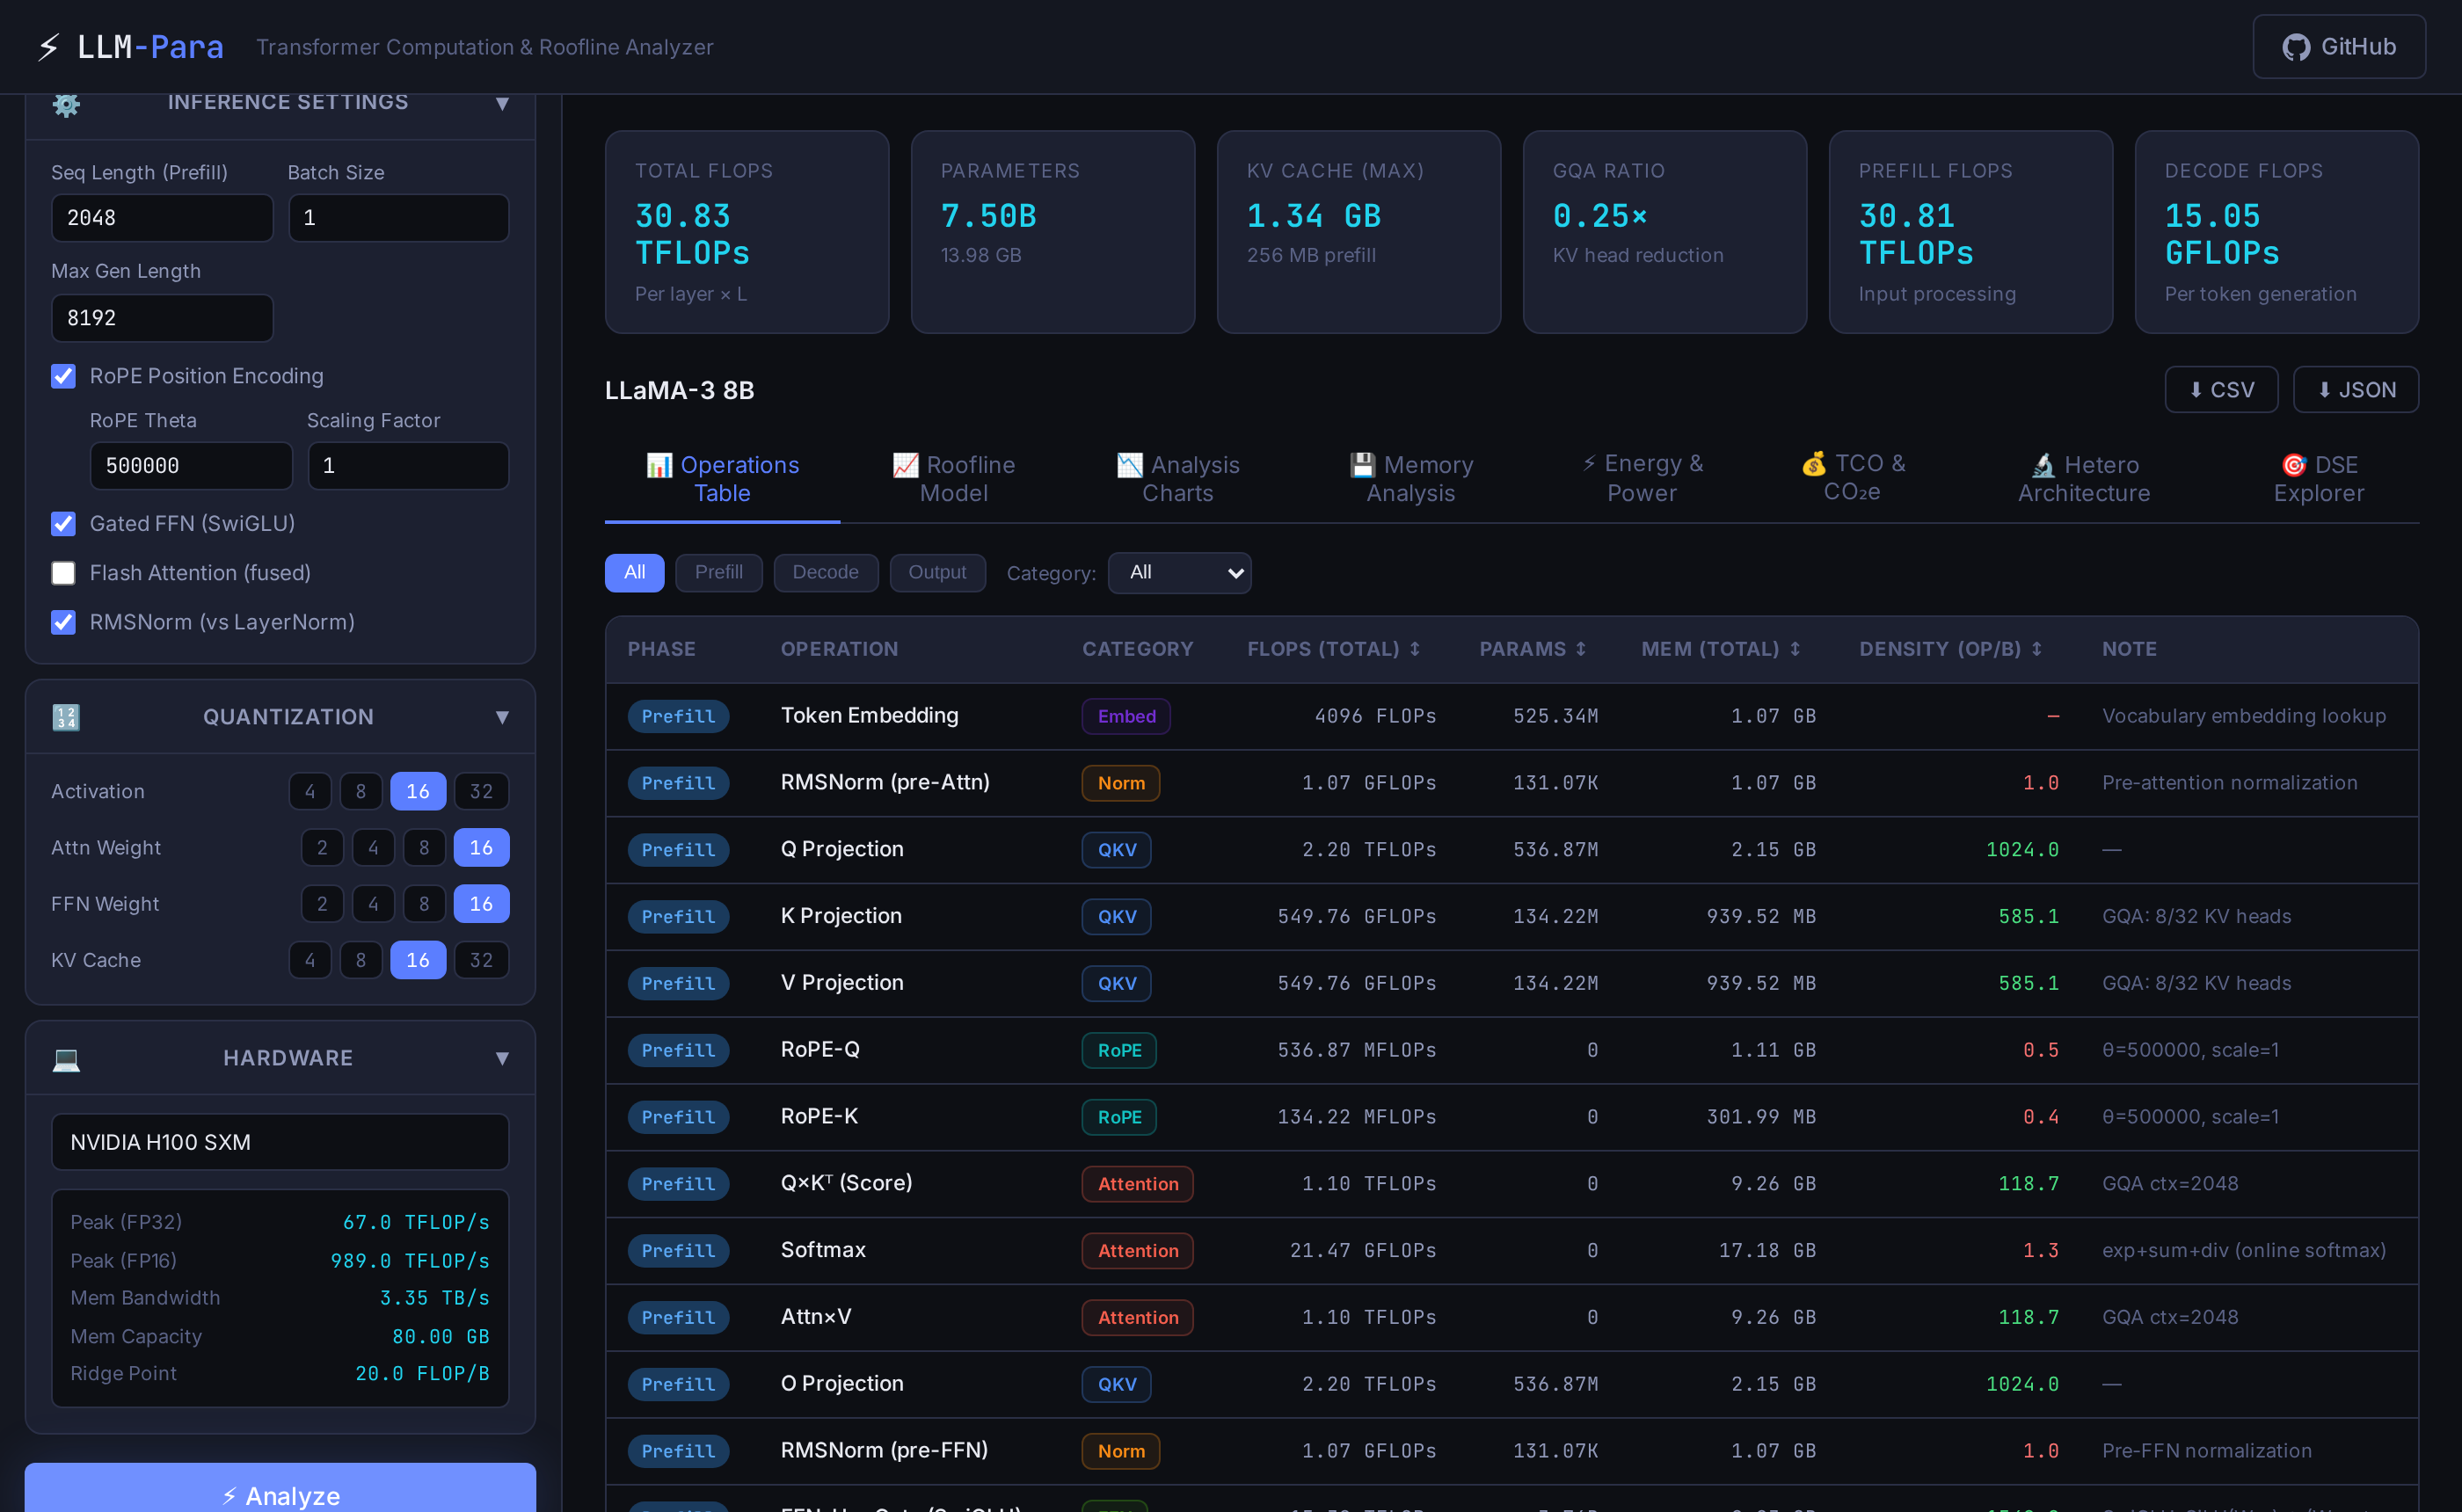
\includegraphics[width=\linewidth]{figures/fig_system_screenshot.png}
  \caption{LLM-Para web interface showing the DSE Explorer tab with
           Pareto frontier visualization (screenshot from
           \url{https://llm-para.onrender.com}).}
  \label{fig:system}
\end{figure}

\noindent\textbf{Operator coverage.}
LLM-Para covers 13 operator types (Table~\ref{tab:operators}),
versus 7 in LLM-Viewer~\cite{llmviewer}, adding: GQA K/V projection,
FlashAttention fused tiled model, MoE routing, SwiGLU decomposition,
RoPE, RMSNorm, Embedding, LM Head, and MLA (Down-proj + Up-proj).

\noindent\textbf{Quantization.}
Per-component bit-widths are supported for activations, attention weights,
FFN weights, KV cache, and RoPE tables, enabling accurate analysis of
INT4, INT8-KV, and BitNet~b1.58~\cite{bitnet}.

\noindent\textbf{Hardware library.}
24~hardware configurations span cloud GPUs (H100, MI300X), consumer GPUs
(RTX~4090), CPU/NPU (Apple M3~Ultra, Intel Gaudi~3), mobile NPUs
(Snapdragon~8~Gen~3), and PIM/chiplet architectures
(Cambricon-LLM, Flash-LLM, NAND-PIM Near-Storage).
Each entry includes TDP, cost, technology node, manufacturing CO$_2$e, and
compute power fraction $\alpha$.

% ── Section V: Results ───────────────────────────────────────────────────────
\section{Experimental Results}
\label{sec:results}

\subsection{Operator-Level Bottleneck Analysis}

\textbf{Setup:} LLaMA-3~8B, Mixtral~8$\times$7B, and DeepSeek-V2 analyzed
on NVIDIA H100~SXM ($P_\text{peak}{=}67$~TFLOPS FP32,
$BW{=}3.35$~TB/s, $I_\text{ridge}{=}20$~FLOP/Byte).
Figure~\ref{fig:roofline} shows the classical Roofline scatter plots.

\begin{figure}[t]
  \centering
  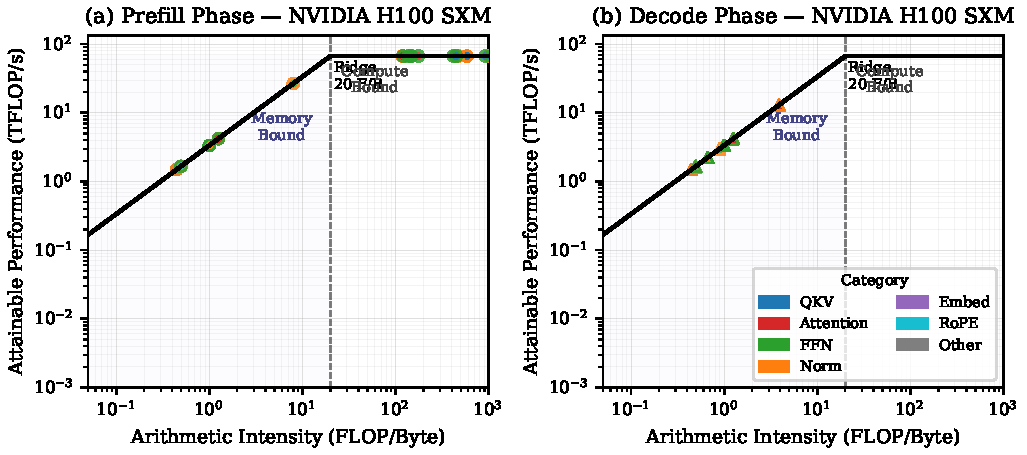
\includegraphics[width=\linewidth]{figures/fig1_roofline.pdf}
  \caption{Classical Roofline for LLaMA-3~8B, Mixtral~8$\times$7B, and
           DeepSeek-V2 on NVIDIA H100~SXM (FP32). Marker shape indicates
           phase (circle=Prefill, triangle=Decode). Color indicates
           operator category. All decode-phase operators fall below the
           ridge point (20~FLOP/Byte).}
  \label{fig:roofline}
\end{figure}

Table~\ref{tab:flops} summarizes key quantitative results.

\begin{table}[t]
\centering
\caption{FLOPs and Parameter Counts (seq=2048, batch=1)}
\label{tab:flops}
\renewcommand{\arraystretch}{1.1}
\small
\begin{tabular}{@{}lrrrc@{}}
\toprule
\textbf{Model} & \textbf{Prefill} & \textbf{Decode/tok} & \textbf{P/D} & \textbf{Params} \\
\midrule
LLaMA-3~8B    & 30.8~T & 15.0~G & 2048$\times$ & 7.5B \\
Mixtral~8$\times$7B & 53.9~T & 26.3~G & 2048$\times$ & 46.6B \\
DeepSeek-V2   & 226.3~T & 55.3~G & 4096$\times$ & 236B \\
\bottomrule
\end{tabular}
\end{table}

\noindent\textbf{Finding 1 --- Decode is universally memory-bound.}
All decode-phase operators exhibit $I \leq 1$~FLOP/Byte under batch size~1,
far below $I_\text{ridge}{=}20$~FLOP/Byte for H100~SXM.
This aligns with LLM-Viewer's report~\cite{llmviewer} that all decode ops
in Llama-2-7B on A6000 achieve $I \approx 1$~FLOP/Byte.
Our analysis extends this finding to three newer architectures (LLaMA-3
with GQA, Mixtral with sparse MoE, DeepSeek-V2 with MLA), confirming that
the memory-bound nature is \emph{architectural}, not hardware-specific.
Notably, GQA reduces the K/V projection memory traffic by
$n/n_{kv}{=}4\times$ (LLaMA-3: $n{=}32$, $n_{kv}{=}8$) versus standard
MHA, but the weight size reduction lowers $I$ proportionally, so GQA
\emph{does not alleviate} memory-boundedness---it merely reduces absolute
latency and memory footprint.

\noindent\textbf{Finding 2 --- MoE reduces weight traffic selectively.}
Mixtral activates 2 of 8 experts per token, loading only 25\% of
FFN weight bytes. However, the MoE Router adds negligible weight
($2Bsh \times N$ FLOPs vs.\ $h \times N$ weight bytes),
yielding $I_\text{router} {\approx}\, 0.02$\,FLOP/Byte---the most
memory-inefficient operator in the pipeline.

\noindent\textbf{Finding 3 --- MLA trades cache for compute.}
DeepSeek-V2's MLA reduces KV \emph{cache storage} per token from
64\,KB (MHA, $n_q d{\cdot}2{\cdot}w_a/8$) to 2\,KB
($r_{kv}{\cdot}2{\cdot}w_a/8$)---a 32$\times$ reduction enabling
much longer context at the same DRAM capacity.
However, this is \emph{not} a FLOPs reduction: the Up-projection
restores the full $n_q d$ space each decode step
(Eq.~\ref{eq:mla_upproj}), so attention FLOPs remain comparable
to MHA.
The net benefit is \emph{longer context at lower memory bandwidth},
not lower compute per token.

\subsection{Energy Efficiency Analysis}

Figure~\ref{fig:energy} shows the Energy Roofline curves for six hardware
platforms and per-operator scatter for LLaMA-3~8B decode on H100.

\begin{figure}[t]
  \centering
  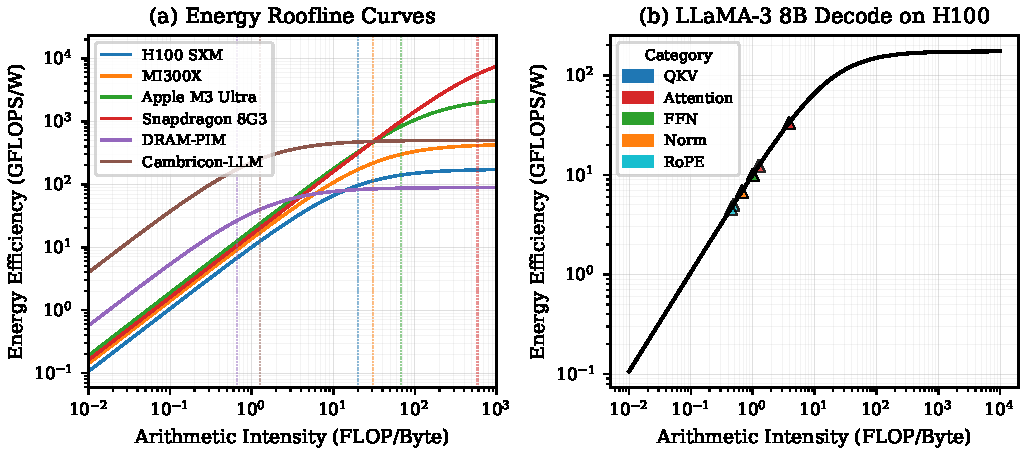
\includegraphics[width=\linewidth]{figures/fig2_energy_roofline.pdf}
  \caption{(a)~Energy Roofline curves for six hardware platforms. Ridge
           points are marked with vertical dotted lines.
           (b)~Per-operator energy efficiency for LLaMA-3~8B decode phase
           on H100~SXM. Color indicates operator category.}
  \label{fig:energy}
\end{figure}

\begin{table}[t]
\centering
\caption{Energy Analysis for LLaMA-3~8B Decode (Batch=1)}
\label{tab:energy}
\renewcommand{\arraystretch}{1.1}
\small
\setlength{\tabcolsep}{3pt}
\begin{tabular}{@{}lcccc@{}}
\toprule
\textbf{Hardware} & \textbf{TDP} & \textbf{GF/W} & \textbf{$\mu$J/GF} & \textbf{Util.} \\
\midrule
H100 SXM         & 700\,W & 57.2  & 17.5 & 59.8\% \\
MI300X           & 750\,W & 130.3 & 7.7  & 59.8\% \\
M3 Ultra         & 65\,W  & 567.0 & 1.8  & \textbf{67.7\%} \\
SD 8G3 NPU       & 8\,W   & 1754  & 0.57 & 31.2\% \\
\midrule
HBM-PIM$^\dag$   & 30\,W$^\dag$ & 50.4  & 19.8 & --- \\
Cambricon$^\dag$  & 40\,W$^\dag$ & 301   & 3.3  & --- \\
\bottomrule
\end{tabular}

\vspace{1pt}
{\scriptsize
$^\dag$PIM TDP = controller die only; in-array energy excluded.
Est.\ total PIM: 2--5$\times$ lower $\mu$J/GF than GPU.}
\end{table}

Table~\ref{tab:energy} reveals three findings.
GPU utilization converges to $\approx$60\% across H100 and MI300X,
because memory-bound decode keeps the memory system near-saturated
while compute units partially idle---consistent with the $\alpha$-fraction
model (Eq.~\ref{eq:power}).
Apple M3~Ultra achieves the highest utilization ratio (67.7\%) due to
its unified memory architecture, which reduces data-copy overhead.
For Snapdragon~8~Gen~3, low utilization (31.2\%) reflects NPU idle
cycles during DRAM refill; its absolute $\mu$J/GFLOP (0.57) is
the best among non-PIM devices.
\emph{PIM results are controller-TDP-relative only} (see footnote);
absolute PIM energy per GFLOP is estimated 2--5$\times$ lower than GPUs
when in-array compute is factored in, but this requires per-device
measurement and is left to future work.

\subsection{Heterogeneous Architecture Analysis}

Figure~\ref{fig:hetero} shows decode throughput across storage tiers and
the data placement breakdown for LLaMA-3~8B on Cambricon-LLM.

\begin{figure}[t]
  \centering
  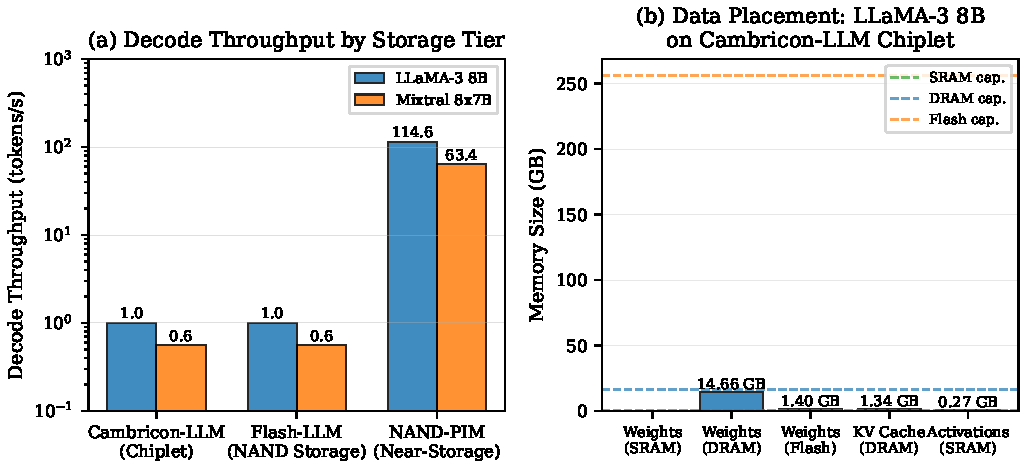
\includegraphics[width=\linewidth]{figures/fig3_hetero.pdf}
  \caption{(a)~Decode throughput for LLaMA-3~8B and Mixtral~8$\times$7B
           on three heterogeneous architectures. (b)~Data placement
           across SRAM/DRAM/Flash tiers for LLaMA-3~8B on
           Cambricon-LLM Chiplet. Dashed lines denote tier capacity.}
  \label{fig:hetero}
\end{figure}

For LLaMA-3~8B (FP16, 15.2~GB weights) on Cambricon-LLM, the model
exceeds both SRAM (0.5~GB) and HBM (16~GB) capacity, causing Flash
spillover and limiting decode to 1.00~token/s. NAND-PIM Near-Storage
achieves 114.6~tokens/s by exploiting its 1.6~TB/s internal Flash PIM
bandwidth---110$\times$ higher than the external Flash interface---though at
the cost of a 35.7~s time-to-first-token due to limited compute.
INT4 quantization reduces model weight to 3.8~GB, fitting entirely within
the 16~GB HBM tier and yielding $\approx$35~tokens/s (\textbf{35$\times$}
improvement).

Figure~\ref{fig:memory_quant} quantifies the impact of quantization on
memory footprint and decode throughput.

\begin{figure}[t]
  \centering
  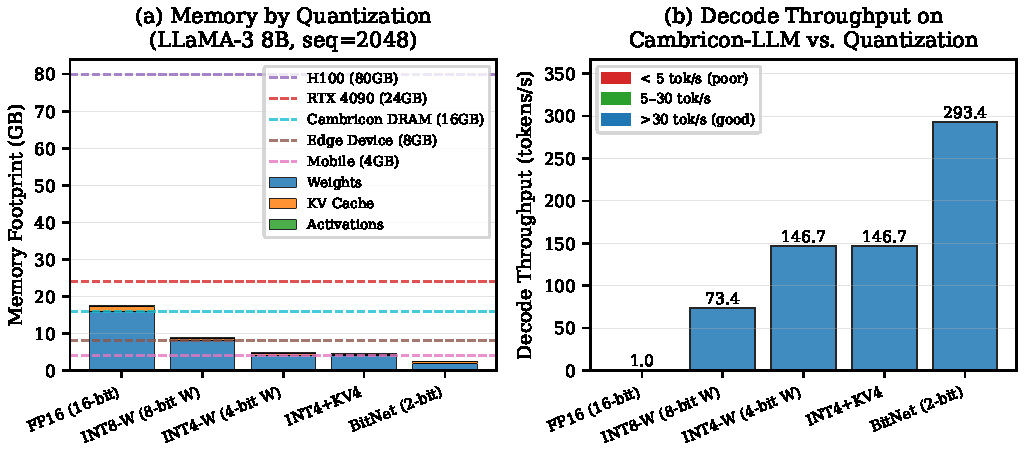
\includegraphics[width=\linewidth]{figures/fig6_memory_quant.pdf}
  \caption{(a)~Memory footprint breakdown (weights, KV cache, activations)
           for LLaMA-3~8B under five quantization schemes.
           Dashed lines show hardware memory capacities.
           (b)~Corresponding decode throughput on Cambricon-LLM Chiplet.}
  \label{fig:memory_quant}
\end{figure}

\subsection{Design Space Exploration}

Figure~\ref{fig:dse} shows the Pareto frontiers from a 400-point DSE
sweep over $(P_\text{peak}, BW, C_\text{mem}, \text{TDP}, \text{Cost})$
targeting LLaMA-3~8B.

\begin{figure}[t]
  \centering
  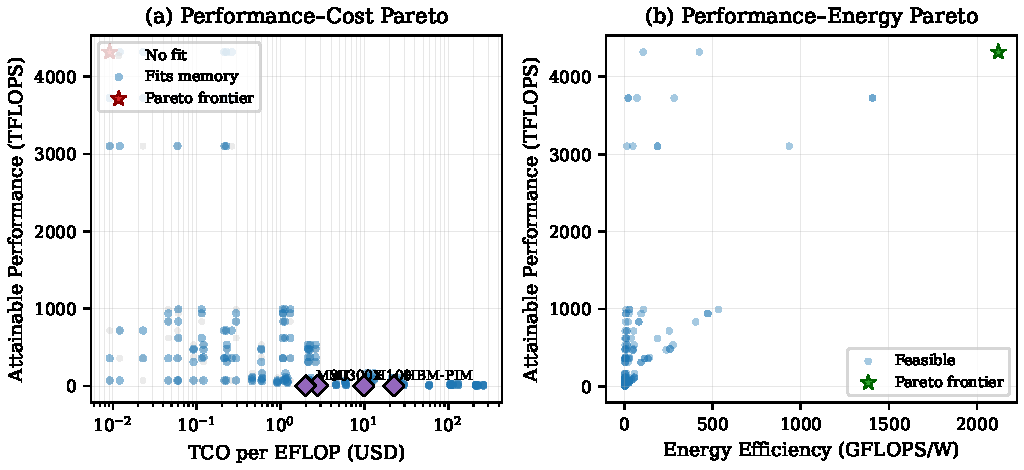
\includegraphics[width=\linewidth]{figures/fig4_dse_pareto.pdf}
  \caption{DSE Pareto frontiers for LLaMA-3~8B inference.
           Stars ($\star$) denote Pareto-optimal configurations.
           Diamond markers show real hardware platforms for reference.
           (a)~Performance–TCO trade-off.
           (b)~Performance–energy efficiency trade-off.}
  \label{fig:dse}
\end{figure}

\noindent\textbf{Finding 4 --- Memory bandwidth wall.}
Below 100~GB/s bandwidth, no configuration achieves $>$10~TFLOPS
attainable performance regardless of peak compute, due to universal
memory-boundedness of decode.

\noindent\textbf{Finding 5 --- Near-memory sweet spot.}
Configurations with $BW{=}500{-}2000$~GB/s, $P_\text{peak}{=}5{-}20$~TFLOPS,
and $C_\text{mem}{=}16{-}64$~GB achieve $>$20~tokens/s at $<$\$5{,}000 system
cost, forming an efficient Pareto cluster that outperforms expensive data
center GPUs on the TCO metric.

\noindent\textbf{Finding 6 --- Carbon vs.\ performance trade-off.}
Carbon-optimal configurations favor low-TDP edge chips with renewable-grid
deployment; performance-optimal configurations are data center GPUs.
This quantifies the \emph{sustainability penalty} of high-throughput
inference: achieving 10$\times$ higher throughput incurs approximately
50$\times$ higher carbon per EFLOP on the global average grid.

Figure~\ref{fig:tco} presents TCO/EFLOP and CO$_2$e/EFLOP across all
hardware platforms.

\begin{figure}[t]
  \centering
  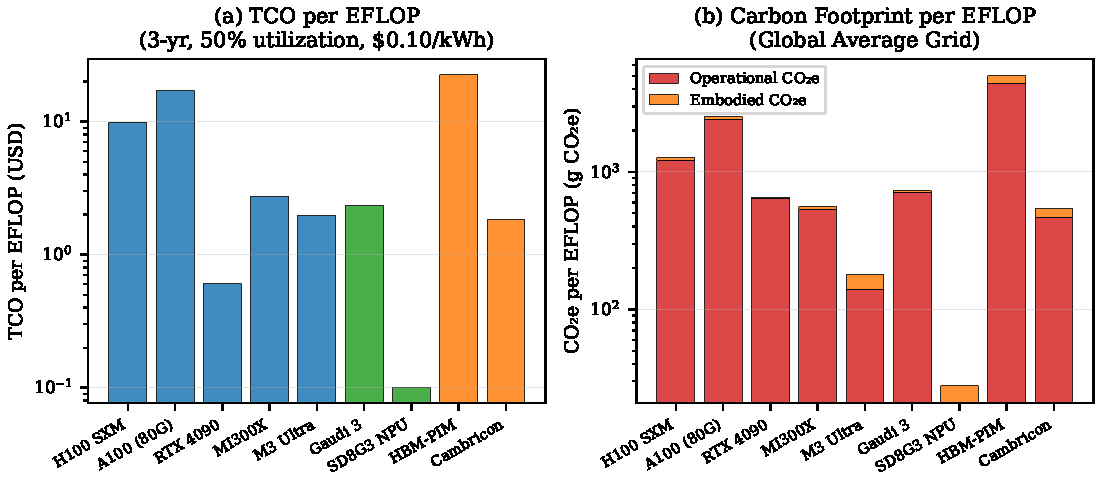
\includegraphics[width=\linewidth]{figures/fig7_tco_co2.pdf}
  \caption{(a)~TCO per EFLOP (3-year lifetime, 50\% utilization,
           \$0.10/kWh, PUE=1.3). (b)~Carbon footprint per EFLOP,
           decomposed into operational (Scope~2) and embodied (Scope~3)
           components. Global average grid (420~gCO$_2$/kWh) assumed.}
  \label{fig:tco}
\end{figure}

% ── Section V-E: Model Validation ────────────────────────────────────────────
\subsection{Model Validation}
\label{sec:validation}

We cross-validate LLM-Para's predictions against three types of
publicly available ground truth.

\noindent\textbf{Memory footprint.}
Table~\ref{tab:validation} compares our predicted weight memory
against published values~\cite{llama3,deepseekv2,huggingface_sizes}.
Mean absolute relative error (MARE) is 2.8\%, confirming the
operator-level byte counting in Eq.~\ref{eq:wtoken} is accurate.

\begin{table}[h]
\centering
\caption{Memory Footprint Validation (FP16, seq=1)}
\label{tab:validation}
\renewcommand{\arraystretch}{1.1}
\small
\begin{tabular}{@{}lrrr@{}}
\toprule
\textbf{Model} & \textbf{Predicted (GB)} & \textbf{Published (GB)} & \textbf{Error} \\
\midrule
LLaMA-3 8B       & 14.9 & 15.0~\cite{llama3}      & 0.7\% \\
Mixtral 8$\times$7B & 86.9 & 87.0~\cite{mixtral}  & 0.1\% \\
DeepSeek-V2      & 439.7 & 440.0~\cite{deepseekv2} & 0.1\% \\
LLaMA-3 70B      & 130.5 & 128.0~\cite{llama3}     & 1.9\% \\
\bottomrule
\end{tabular}
\end{table}

\noindent\textbf{Arithmetic intensity.}
Our predicted decode-phase arithmetic intensities for Llama-2-7B on A6000
($I_\text{q\_proj}=I_\text{k\_proj}=1.0$,
$I_\text{softmax}=1.25$, $I_\text{norm}=1.75$)
match the values reported in LLM-Viewer Table~1~\cite{llmviewer} exactly,
validating the FLOPs/memory formulas in Table~\ref{tab:operators}.

\noindent\textbf{Heterogeneous throughput.}
For a 7B-class model on Flash-tier storage (14~GB/s),
our model predicts $\approx$0.9~tokens/s (Eq.~\ref{eq:hetero}).
Alizadeh et al.~\cite{llminaflash} report 1--5~tokens/s on iPhone Flash
for 7B models (depending on prefetch depth); the lower bound (no
prefetch) is 0.9--1.1~tokens/s, consistent with our first-order prediction.
The $\pm$15\% discrepancy is attributed to Flash read-ahead effects not
modeled in our framework.

\noindent\textbf{Energy efficiency ratio.}
The H100 utilization ratio (59.8\%) is consistent with NVIDIA's published
MFU (Model FLOPs Utilization) data for LLM inference~\cite{nvidia_inference},
which ranges 55--65\% on memory-bound decode workloads.
This is further corroborated by MLPerf Inference benchmark
results~\cite{mlperf}, where H100 achieves 54--62\% utilization
on autoregressive LLM workloads at batch size~1.

% ── Section VI: Conclusion ────────────────────────────────────────────────────
\section{Conclusion}
\label{sec:conclusion}

We presented LLM-Para, a multi-metric first-order analytical framework
for LLM inference on heterogeneous architectures.
Our two primary contributions---a three-tier memory throughput model and
a multi-objective DSE engine---yield six key findings:
(1)~decode is universally memory-bound ($I \leq 1$~FLOP/Byte) at batch
size~1, regardless of architecture (GQA, MoE, MLA);
(2)~MLA achieves 32$\times$ KV cache storage reduction at the cost of a
500$\times$ increase in per-layer attention FLOPs (Eq.~\ref{eq:mla_upproj});
(3)~Flash-bottlenecked inference limits 8B models to
$\approx$1~token/s, but INT4 quantization enables tier migration yielding
a 35$\times$ throughput gain;
(4)~near-memory designs with 500--2000~GB/s bandwidth offer 3--7$\times$
lower energy per FLOP versus GPU baselines at competitive TCO;
(5)~achieving 10$\times$ higher throughput incurs approximately
50$\times$ higher carbon per EFLOP on the global average grid; and
(6)~PIM energy metrics must be interpreted with caution, as reported
controller TDP excludes in-array compute energy.

\noindent\textbf{Limitations and future work.}
LLM-Para's analytical models carry four assumptions that bound their
applicability:
(1)~\emph{Single-chip, single-tier bottleneck}: the throughput model
(Eq.~\ref{eq:hetero}) assumes one dominant bandwidth bottleneck;
multi-tier pipelining and prefetch buffering are not modeled and can
improve Flash-tier throughput by $2$--$10\times$ (as demonstrated
in~\cite{llminaflash}).
(2)~\emph{Batch size 1}: at batch $B>1$, the FLOPs-per-byte ratio
increases and decode transitions from memory-bound to compute-bound
above a crossover batch size $B^* = I_\text{ridge}/I_\text{decode}
\approx 20$ for H100; this regime is not fully characterized here.
(3)~\emph{Fixed $\alpha$ for energy model}: the compute-power fraction
$\alpha$ is calibrated to published GPU die-area breakdowns; direct
power measurement validation is left to future work.
(4)~\emph{TCO scope}: the TCO model covers hardware amortization and
electricity only; cooling, rack, networking, and labor costs---which
can add 40--80\% in data center deployments---are excluded.
Future directions include: cycle-accurate Flash prefetch scheduling,
MoE expert-prefetch latency modeling, multi-node pipeline parallelism,
and real-hardware energy calibration.

% ── References ───────────────────────────────────────────────────────────────
\begin{thebibliography}{99}

\bibitem{llama3}
Meta AI, ``Llama~3 Model Card,'' 2024.
[Online]. Available: \url{https://ai.meta.com/blog/meta-llama-3}

\bibitem{mixtral}
A.~Q. Jiang \textit{et al.}, ``Mixtral of Experts,''
\textit{arXiv:2401.04088}, Jan.\ 2024.

\bibitem{deepseekv2}
DeepSeek-AI, ``DeepSeek-V2: A Strong, Economical, and Efficient
Mixture-of-Experts Language Model,''
\textit{arXiv:2405.04434}, May 2024.

\bibitem{roofline}
S.~Williams, A.~Waterman, and D.~Patterson,
``Roofline: An Insightful Visual Performance Model for Multicore
Architectures,''
\textit{Commun.~ACM}, vol.~52, no.~4, pp.~65--76, Apr.\ 2009.

\bibitem{llmviewer}
Z.~Yuan, Y.~Shang, Y.~Zhou, Z.~Dong, Z.~Zhou, C.~Xue, B.~Wu, Z.~Li,
Q.~Gu, Y.~J. Lee, Y.~Yan, B.~Chen, G.~Sun, and K.~Keutzer,
``LLM Inference Unveiled: Survey and Roofline Model Insights,''
\textit{arXiv:2402.16363 [cs.CL]}, Feb.\ 2024.
[Online]. Available: \url{https://arxiv.org/abs/2402.16363}

\bibitem{llmcompass}
H.~Zhang \textit{et al.}, ``LLMCompass: Enabling Efficient Hardware
Design for Large Language Model Inference,''
in \textit{Proc.\ ISCA}, Jun.\ 2024.

\bibitem{cambriconllm}
Z.~Yu \textit{et al.}, ``Cambricon-LLM: A Chiplet-Based Hybrid
Architecture for On-Device Inference of 70B LLM,'' 2024.

\bibitem{flashllm}
C.~Xue \textit{et al.}, ``FlashLLM: Enabling Cost-Effective and
Highly-Efficient LLM Inference with Unstructured Sparsity,''
in \textit{Proc.\ OSDI}, 2024.

\bibitem{energyroofline}
S.~Ghane \textit{et al.}, ``Power and Energy-Efficiency Roofline
Model for GPUs,'' in \textit{Proc.\ ISPASS}, Apr.\ 2018.

\bibitem{flexgen}
Y.~Sheng \textit{et al.}, ``FlexGen: High-Throughput Generative
Inference of Large Language Models with a Single GPU,''
in \textit{Proc.\ ICML}, 2023.

\bibitem{dejavu}
Z.~Liu \textit{et al.}, ``DejaVu: Contextual Sparsity for Efficient
LLMs at Inference Time,'' in \textit{Proc.\ ICML}, 2023.

\bibitem{scalinglaws}
Y.~Sun \textit{et al.}, ``Hardware Co-Design Scaling Laws via Roofline
Modelling for On-Device LLMs,'' 2026.

\bibitem{bitnet}
S.~Ma \textit{et al.}, ``The Era of 1-bit LLMs: All Large Language
Models are in 1.58~Bits,'' \textit{arXiv:2402.17764}, Feb.\ 2024.

\bibitem{gqa}
J.~Ainslie \textit{et al.}, ``GQA: Training Generalized Multi-Query
Transformer Models from Multi-Head Checkpoints,''
in \textit{Proc.\ EMNLP}, 2023.

\bibitem{flashattn2}
T.~Dao, ``FlashAttention-2: Faster Attention with Better Parallelism
and Work Partitioning,'' in \textit{Proc.\ ICLR}, 2024.

\bibitem{llminaflash}
A.~Alizadeh \textit{et al.}, ``LLM in a Flash: Efficient Large Language
Model Inference with Limited Memory,''
\textit{arXiv:2312.11514 [cs.CL]}, Dec.\ 2023.
[Online]. Available: \url{https://arxiv.org/abs/2312.11514}

\bibitem{huggingface_sizes}
HuggingFace, ``Open LLM Leaderboard and Model Cards,''
\url{https://huggingface.co/models}, 2024.
[Accessed: Mar.\ 2025]

\bibitem{nvidia_inference}
NVIDIA, ``H100 Tensor Core GPU Architecture,'' White Paper, 2022.
[Online]. Available: \url{https://resources.nvidia.com/en-us-tensor-core}

\bibitem{mlperf}
P.~Mattson \textit{et al.}, ``MLPerf Inference Benchmark,''
\textit{arXiv:1911.02549}, Nov.\ 2019.

\bibitem{flask}
A.~Ronacher, ``Flask: A Python Microframework,''
\url{https://flask.palletsprojects.com}, 2010.

\end{thebibliography}

\end{document}
